\documentclass[12pt, letterpaper]{article}
\date{\today}
\usepackage[margin=1in]{geometry}
\usepackage{amsmath}
\usepackage{hyperref}
\usepackage{cancel}
\usepackage{amssymb}
\usepackage{fancyhdr}
\usepackage{pgfplots}
\usepackage{booktabs}
\usepackage{pifont}
\usepackage{amsthm,latexsym,amsfonts,graphicx,epsfig,comment}
\pgfplotsset{compat=1.16}
\usepackage{xcolor}
\usepackage{tikz}
\usetikzlibrary{shapes.geometric}
\usetikzlibrary{arrows.meta,arrows}
\newcommand{\Z}{\mathbb{Z}}
\newcommand{\N}{\mathbb{N}}
\newcommand{\R}{\mathbb{R}}
\newcommand{\Po}{\mathcal{P}}

\author{Alex Valentino}
\title{Challange problem set 2}
\pagestyle{fancy}
\renewcommand{\headrulewidth}{0pt}
\renewcommand{\footrulewidth}{0pt}
\fancyhf{}
\rhead{
	Challange problem set 2 \\
	292	
}
\lhead{
	Alex Valentino\\
}

\begin{document}
\begin{enumerate}
	\item 
	\begin{align*}
		\Vec{x}'' &= (\Vec{x}_0 + \sum_{j = 1}^4 \Vec{x}_j)''\\
		&= \Vec{x}_0'' + \sum_{j = 1}^4 \Vec{x}_j''\\
		&= -K \Vec{x}_0 + \sum_{j = 1}^4  (-K \Vec{x}_j + \Vec{f}_j)\\
		&= -K(\Vec{x}_0 + \sum_{j = 1}^4 \Vec{x}_j) + \sum_{j = 1}^4 \Vec{f}_j\\
		&= -K \Vec{x} + \sum_{j = 1}^4 \Vec{f}_j
	\end{align*}
	Therefore we have found a solution to the differential equation $\Vec{x}'' = -K \Vec{x} + \sum_{j = 1}^4 \Vec{f}_j$.
	\item The matrix $K = \begin{bmatrix}
	3 & 2\\ 2 & 6
	\end{bmatrix}$ has the characteristic polynomial $\lambda^2 -9 \lambda + 14$, thus $K$ has eigenvalues $\mu_1 = 7, \mu_2 = 2$.  These correspond with the normalized eigenvectors $\Vec{v}_1 = \frac{1}{\sqrt{5}} \begin{bmatrix}1 \\ 2	\end{bmatrix}$,
	 $\Vec{v}_2 = \frac{1}{\sqrt{5}} \begin{bmatrix}2 \\ -1	\end{bmatrix}$.  Let $V = \begin{bmatrix} 
	 \Vec{v}_1 &\Vec{v}_2\end{bmatrix}$, and $D = \begin{bmatrix} 7 & 0 \\ 0 & 2 \end{bmatrix}$.\\  Therefore $K = V D V^{-1} = 
	 \frac{1}{5}\begin{bmatrix} 1 & 2 \\ 2 & -1\end{bmatrix}\begin{bmatrix}7 & 0 \\ 2 & 0 \end{bmatrix} \begin{bmatrix}-1 & -2\\ -2 & 1\end{bmatrix}$.  
	 Since we have shown that $K$ diagonalizes, then we can show that $V^{-1}\Vec{x}_0'' =  -D V^{-1}\Vec{x}_0$:
	 $$
		V^{-1}\Vec{x}_0'' = 	-V^{-1} K \Vec{x}_0 = - V^{-1} V D V^{-1} \Vec{x}_0 = -D V^{-1}\Vec{x}_0.
	 $$
	 Since $V^{-1}$ is a matrix then $V^{-1} \Vec{x}_0 (0) = V^{-1}(1,2),V^{-1} \Vec{x}_0' (0) = V^{-1}(1,1)$ is just the definition of matrix multiplication.\\
	 Similarly for $V^{-1} \Vec{x}_j'' = - D V^{-1} \Vec{x}_j + V^{-1} \Vec{f}_j$,
	 $$
			 V^{-1}\Vec{x}_j'' = 	-V^{-1} K \Vec{x}_j + V^{-1} \Vec{f}_j = - V^{-1} V D V^{-1} \Vec{x}_j  + V^{-1} \Vec{f}_j = -D V^{-1}\Vec{x}_j + V^{-1} \Vec{f}_j.  
	 $$
	 And once again since the initial conditions are vectors you may simply multiply them.
	 \item 
	 \begin{align*}
	 	y''(t) &= (y(0) \cos(\sqrt{\kappa} t) + \frac{y'(0)}{\sqrt{\kappa}}\sin(\sqrt{\kappa} t) + \frac{1}{\sqrt{\kappa}}\int_0^t \sin(\sqrt{\kappa} (t-s)) g(s) ds)''\\
	 	&= y(0) \cos(\sqrt{\kappa} t)'' + \frac{y'(0)}{\sqrt{\kappa}}\sin(\sqrt{\kappa} t)'' + \frac{1}{\sqrt{\kappa}}(\int_0^t \sin(\sqrt{\kappa} (t-s)) g(s) ds)''\\
	 	&= -\kappa y(0) \cos(\sqrt{\kappa} t) - \sqrt{\kappa} y'(0) \sin(\sqrt{\kappa} t) + (\int_0^t \cos(\sqrt{\kappa} (t-s)) g(s) ds)'\\
	 	&= -\kappa y(0) \cos(\sqrt{\kappa} t) - \sqrt{\kappa} y'(0) \sin(\sqrt{\kappa} t) + g(t) - \sqrt{\kappa} \int_0^t \sin(\sqrt{\kappa} (t-s)) g(s) ds \\ 
	 	&\text{(using the Leibniz integral rule)}\\
	 	&= -\kappa(y(0) \cos(\sqrt{\kappa} t) + \frac{y'(0)}{\sqrt{\kappa}}\sin(\sqrt{\kappa} t) + \frac{1}{\sqrt{\kappa}}\int_0^t \sin(\sqrt{\kappa} (t-s)) g(s) ds) + g(t) \\
	 	&= -\kappa y(t) + g(t)
	 \end{align*}
	 \item To solve for $\Vec{x}_0$, since we know what the eigenvectors are and we have a formula for solving the equation the equation $w_j' = -\mu_j w_j$ where 
	 $$
	 	w_j (t) = (\Vec{x}_0 (0) \cdot \Vec{v}_j)\cos(\sqrt{\mu_j} t) + \frac{(\Vec{x}_0' (0) \cdot \Vec{v}_j)}{\sqrt{\kappa_j}} \sin(\sqrt{\mu_j} t)	 
	 $$
	 with $\Vec{x}_0 = \sum_{j=1}^2 w_j \Vec{u}_j$.  Therefore 
	 $ w_1 = \frac{3 \sin \left(\sqrt{7} t\right)}{\sqrt{35}}+\sqrt{5} \cos \left(\sqrt{7}
   t\right),w_2 = -\frac{\sin \left(\sqrt{2} t\right)}{\sqrt{10}}$.
   Thus 
   $$
	\Vec{x}_0 (t) = \left(\frac{1}{5} \sqrt{2} \sin (\sqrt{2} t)+\frac{3 \sin
   (\sqrt{7} t)}{5 \sqrt{7}}+\cos (\sqrt{7} t),-\frac{\sin
   (\sqrt{2} t)}{5 \sqrt{2}}+\frac{6 \sin (\sqrt{7} t)}{5
   \sqrt{7}}+2 \cos (\sqrt{7} t)\right)   
   $$\\
    To solve the general equation $\Vec{x}_i = -K \Vec{x}_i + \Vec{f}_i$, since $\Vec{f}_i = \cos (\phi_i + \omega_i t) \Vec{u}_i$, then we have a solution for each component 
   $w_{i,j} = (\Vec{x}_i (0) \cdot \Vec{v}_j)\cos(\sqrt{\mu_j} t) + \frac{(\Vec{x}_i' (0) \cdot \Vec{v}_j)}{\sqrt{\kappa_j}} \sin(\sqrt{\mu_j} t) + \frac{2(\Vec{u}_i\cdot \Vec{v}_j)}{\sqrt{\mu_j}}\left( \sin(\phi_{i} - \xi_{i,j} t) \frac{\sin(\eta_{i,j} t)}{\eta_{i,j}}+\sin(\phi_{i} + \eta_{i,j} t) \frac{\sin(\xi_{i,j} t)}{\xi_{i,j}} \right)$
   where $\xi_{i,j} = \frac{ \sqrt{\mu_j} + \omega_i }{2},\eta_{i,j} = \frac{ \sqrt{\mu_j}-\omega_i}{2}$.\\
   Since for all $i \in [4], \Vec{x}_i (0) = \Vec{x}_i' = (0,0)$, then our solution $\Vec{x}_i$ for each $i\in [4]$ is:
   $$
   \Vec{x}_i = \sum_{j=1}^2  \frac{2(\Vec{u}_i\cdot \Vec{v}_j)}{\sqrt{\mu_j}}\left( \sin(\phi_{i} - \xi_{i,j} t) \frac{\sin(\eta_{i,j} t)}{\eta_{i,j}}+\sin(\phi_{i} + \eta_{i,j} t) \frac{\sin(\xi_{i,j} t)}{\xi_{i,j}} \right) \Vec{v}_j.
   $$
   \item $\Vec{f}_1 = \cos(\omega_1)(1,3)$, thus $\phi_1 = 0, \Vec{u}_1 = (1,3)$.  Therefore by our formula:\\
   $
   \Vec{x}_1 = \left( \frac{4}{5} \omega_1 \left(\frac{\sqrt{2} \left(\cos
   \left(\sqrt{2} t\right)-\cos (t \omega_1)\right)}{\omega_1^2-2}+\frac{\sqrt{7} \left(\cos (t \omega_1)-\cos \left(\sqrt{7}
   t\right)\right)}{\omega_1^2-7}\right),\frac{4}{5} \omega_1
   \left(\frac{\cos (t \omega_1)-\cos \left(\sqrt{2} t\right)}{\sqrt{2}
   \left(\omega_1^2-2\right)}+\frac{2 \sqrt{7} \left(\cos (t
   \omega_1)-\cos \left(\sqrt{7} t\right)\right)}{\omega_1^2-7}\right)\right)
   $
   \item $\Vec{f}_2 = \sin (\omega_2 t) (1,-1)$, thus $\phi_2 = -\frac{\pi}{2}, \Vec{u}_2 = (1,-1)$.
   Therefore by our formula:\\
   $
   \Vec{x}_2 = (\frac{2}{35} \left(\frac{98 \left(2 \sin \left(\sqrt{2} t\right)-\sqrt{2}
   \omega_2 \sin (t \omega_2)\right)}{\omega_2^2-2}+\frac{2 \left(7 \sin \left(\sqrt{7} t\right)-\sqrt{7}\omega_2 \sin (t \omega_2)\right)}{\omega_2^2-7}\right),$\\
   $
   \frac{14
   \left(\sqrt{2} \omega_2 \sin (t \omega_2)-2 \sin
   \left(\sqrt{2} t\right)\right)}{5 \left(\omega_2^2-2\right)}+\frac{8
   \left(7 \sin \left(\sqrt{7} t\right)-\sqrt{7} \omega_2 \sin (t
   \omega_2)\right)}{35 \left(\omega_2^2-7\right)})
   $
   \item $\Vec{f}_3 = \sin (\omega_3 t) (3,-1)$, thus $\phi_3 = -\frac{\pi}{2}, \Vec{u}_3 = (3,-1)$
    Therefore by our formula:\\
    $
	\Vec{x}_3 = \frac{4}{35} \left(\frac{21 \left(2 \sin \left(\sqrt{2} t\right)-\sqrt{2}
   \omega_3 \sin (t \omega_3)\right)}{\omega_3^2-2}+\frac{\sqrt{7} \omega_3 \sin (t \omega_3)-7 \sin
   \left(\sqrt{7} t\right)}{\omega_3^2-7}\right),$\\
   $\frac{6 \left(\sqrt{2}
   \omega_3 \sin (t \omega_3)-2 \sin \left(\sqrt{2}
   t\right)\right)}{5 \left(\omega_3^2-2\right)}+\frac{8 \left(\sqrt{7}
   \omega_3 \sin (t \omega_3)-7 \sin \left(\sqrt{7}
   t\right)\right)}{35 \left(\omega_3^2-7\right)}
    $
    \item  $\Vec{f}_4 = \cos(\omega_4)(1,0)$, thus $\phi_1 = 0, \Vec{u}_1 = (1,0)$.  Therefore by our formula:\\
    $\Vec{x}_4 = \frac{4}{35} \omega_4 \left(\frac{14 \sqrt{2} \left(\cos (t
   \omega_4)-\cos \left(\sqrt{2} t\right)\right)}{\omega_4^2-2}+\frac{\sqrt{7} \left(\cos (t \omega_4)-\cos \left(\sqrt{7}
   t\right)\right)}{\omega_4^2-7}\right),$\\
   $\frac{4}{35} \omega_4
   \left(\frac{7 \sqrt{2} \left(\cos \left(\sqrt{2} t\right)-\cos (t \omega_4)\right)}{\omega_4^2-2}+\frac{2 \sqrt{7} \left(\cos (t
   \omega_4)-\cos \left(\sqrt{7} t\right)\right)}{\omega_4^2-7}\right)$
   \item $\Vec{x}$ will experience resonance when any of the forcing function frequencies are either $\pm \sqrt{2}$ or $\pm \sqrt{7}$.  If one takes $\omega_3 $ to approach $ \sqrt{2}$ then the limit evaluates to: \\
   $
	\lim_{t \to \sqrt{2}} \Vec{x}_3 (t) = (-\frac{2}{175} \left(\left(105+2 \sqrt{14}\right) \sin \left(\sqrt{2}
   t\right)-14 \sin \left(\sqrt{7} t\right)+105 \sqrt{2} t \cos \left(\sqrt{2}
   t\right)\right),$\\
   $\frac{1}{175} \left(\left(105-8 \sqrt{14}\right) \sin
   \left(\sqrt{2} t\right)+56 \sin \left(\sqrt{7} t\right)+105 \sqrt{2} t \cos
   \left(\sqrt{2} t\right)\right))  
   $
   \item 
   \begin{enumerate}
		\item[$\Vec{x}_0$] First component\\
		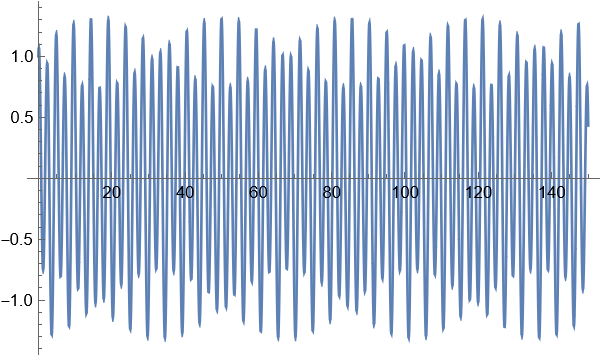
\includegraphics[scale=1.0]{x0com1.png}\\
		Second component\\
		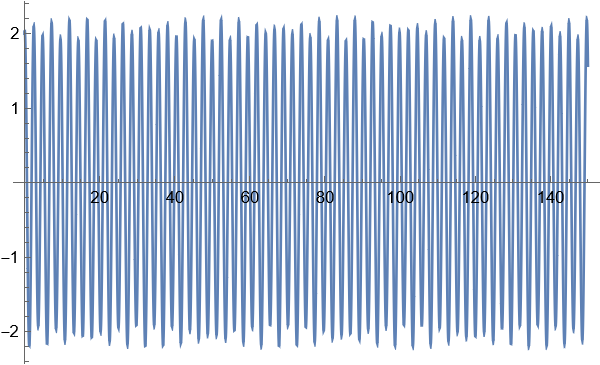
\includegraphics[scale=1.0]{x0com2.png}
		\item[$\Vec{x}_1$] First component\\
		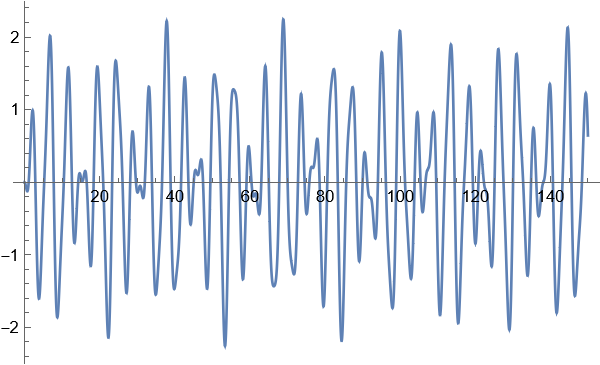
\includegraphics[scale=1.0]{x1com1.png}\\
		Second component\\
		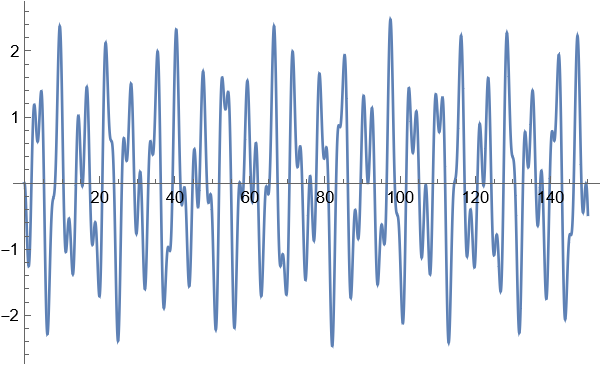
\includegraphics[scale=1.0]{x1com2.png}
		\item[$\Vec{x}_2$] First component\\
		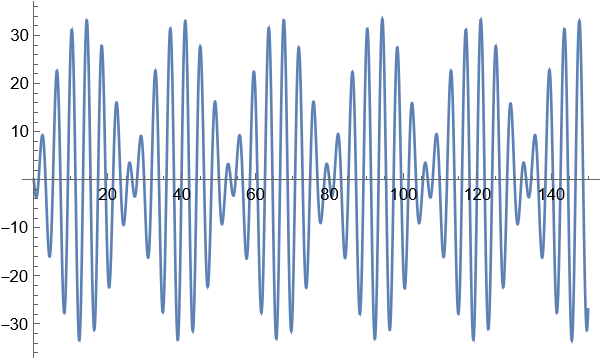
\includegraphics[scale=1.0]{x2com1.png}\\
		Second component\\
		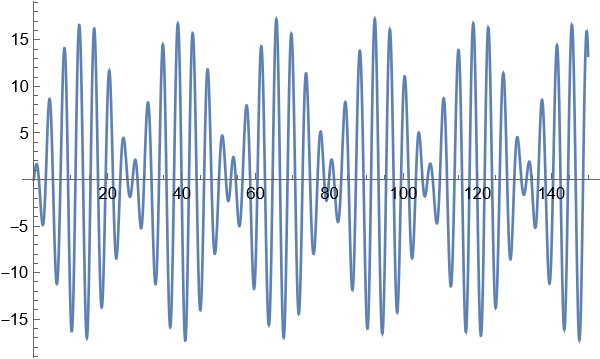
\includegraphics[scale=1.0]{x2com2.png}
		\item[$\Vec{x}_3$] First component\\
		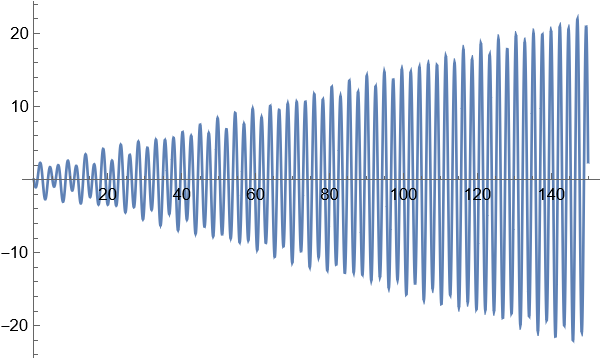
\includegraphics[scale=1.0]{x3com1.png}\\
		Second component\\
		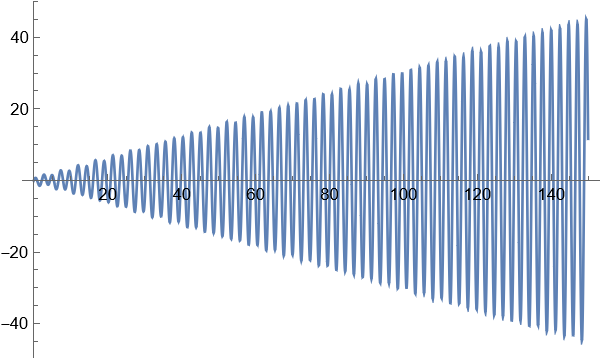
\includegraphics[scale=1.0]{x3com2.png}
		\item[$\Vec{x}_4$] First component\\
		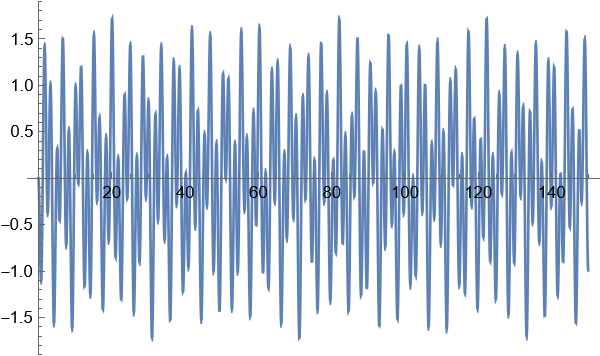
\includegraphics[scale=1.0]{x4com1.png}\\
		Second component\\
		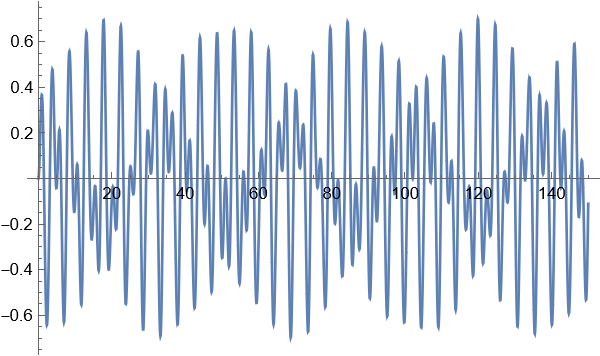
\includegraphics[scale=1.0]{x4com2.png}\\
		Clearly $\Vec{x}_3$ is the dominating term, as $2.65 \approx \sqrt{7}$, therefore it's behavior is approaching resonant.  
   \end{enumerate}
\end{enumerate}
\end{document}